%===============================================
\section{Measurement of Higgs boson couplings}
\frame{\tableofcontents[currentsection]}

%%=================================================================================
\begin{frame}{Simplified Template Cross Section (STXS) framework}
  \centering
  \includegraphics[width=0.8\linewidth]{HTSX.pdf}\\
  Replace signal strengths ($\mu=\frac{\sigma^{exp}}{\sigma^{th}}$) by cross-section in exclusive phase space regions.
\end{frame}
%%=================================================================================
\begin{frame}{Couplings measurement strategy}

  \begin{minipage}{0.49\linewidth}
  {\bf Inclusive selection }
  \begin{itemize}
  \item 2 tight photons
  \item $\frac{p_T^\gamma}{m_{\gamma\gamma}}>0.35 (0.25)$
  \item $|\eta|\in [0, 1.137]  \cup [1.52, 2.37]$
  \item $m_{\gamma\gamma} \in [105, 160]$ GeV
  \end{itemize}
  \end{minipage}
  \hfill
  \begin{minipage}{0.49\linewidth}
    {\bf Dataset properties}  

    \begin{itemize}
    \item $\sim$ 330k events
    \item $42\%$ signal efficiency
    \item $\simeq 1730$ expected signal yield
    \end{itemize}
  \end{minipage}
  \vfill
  {\bf Analysis strategy } 
  \begin{itemize}
  \item Define reconstructed categories targetting specific truth bin.
  \item Measure acceptance of each category wrt truth bins.
  \item Evaluate systematics effects on signal model.
  \item Combined fit of $m_{\gamma\gamma}$ distribution with signal+bkg model.
  \end{itemize}

\end{frame}
%%=================================================================================
\begin{frame}{Reconstructed categories}
  \begin{minipage}{0.49\linewidth}
      \includegraphics[width=\linewidth]{ATL-COM-PHYS-2016-1784_flowchart-eps-converted-to.pdf}
  \end{minipage}
  \hfill
  \begin{minipage}{0.49\linewidth}
    Optimised sensitivity to :
    \begin{itemize}
    \item rare processes
    \item truth bins
    \end{itemize}
    \includegraphics[width=\linewidth]{ATLAS-CONF-2017-045_4t.pdf}
  \end{minipage}
\end{frame}
%%=================================================================================
\begin{frame}{Truth bin distribution}
  \begin{minipage}{0.6\linewidth}
      \includegraphics[width=\linewidth]{ATL-COM_PHYS_2016-1784_purity_2D.pdf}
  \end{minipage}
  \hfill
  \begin{minipage}{0.39\linewidth}
    \begin{itemize}
    \item \textcolor{blue}{Columns : distribution of events of a given category over the truth bins.}
    \item Rectangles : process optimised categories
    \end{itemize}
  \end{minipage}
  
  \centering
  \textcolor{red}{\bf Good performances of process targetting}
\end{frame}
%%=================================================================================
\begin{frame}{Background parametrization}
  \begin{minipage}{0.45\linewidth}
    \includegraphics[width=\linewidth]{ATLAS-CONF-2017-045_3fa.pdf}
  \end{minipage}
  \hfill
  \begin{minipage}{0.45\linewidth}
    \begin{itemize}
    \item MC not reliable for MC description
    \item Shape fitted on data
    \item Spurious signal evaluated for selection of functional form.
    \end{itemize}
  \end{minipage}\\
  \includegraphics[width=0.9\linewidth]{ATL-COM-PHYS-2016-1784_52f.pdf}
\end{frame}
%%=================================================================================
\begin{frame}{Calibration uncertainties methodology}
  \begin{minipage}{0.49\linewidth}
    For a given systematic source :
    \begin{itemize}
    \item Create distributions of \\ $m_{\gamma\gamma}^{nom}$, $m_{\gamma\gamma}^{up}$, $m_{\gamma \gamma}^{down}$
    \item Fit main parameter of the systematic with DSCB :
      \begin{itemize}
      \item Fit  $m_{\gamma\gamma}\in[105,160]$GeV
      \item Fixing $n_{high}=5$ and $n_{low}=9$
      \item Fixing $\alpha_{high}=\hat{\alpha}_{high}^{nom}$, $\alpha_{low}^{nom}=\hat{\alpha}_{low}^{nom}$, $X=\hat{X}^{nom}$
%        \item Fixing secondary parameter to nominal fitted values.
      \end{itemize}
      \item Systematic variation : $\frac{X^{fluct}}{X^{nom}}-1$, $X\in \{\mu , \sigma\}$
      \end{itemize}
    \end{minipage}
    \hfill
    \begin{minipage}{0.49\linewidth}
      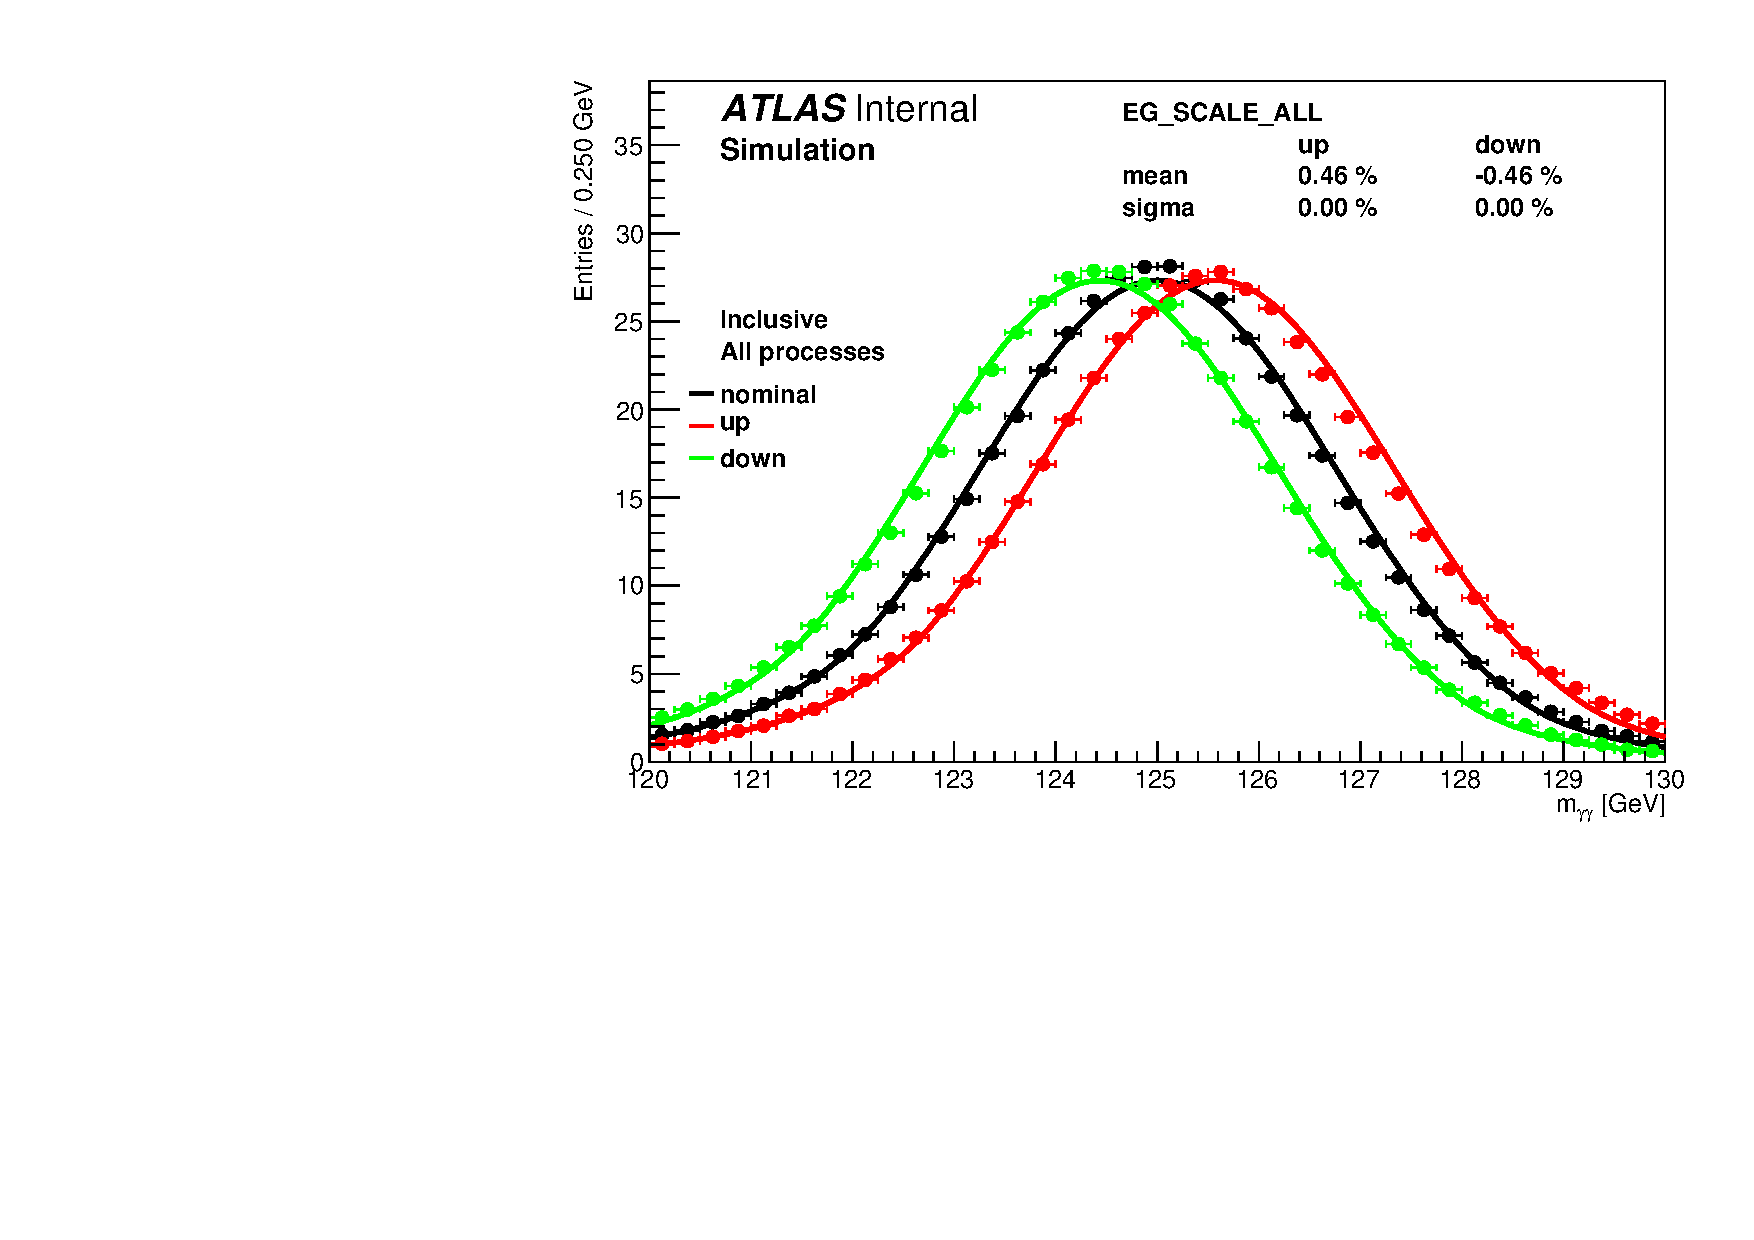
\includegraphics[width=\linewidth]{Figures/h013_EG_SCALE_ALL_0.pdf}
    \end{minipage}
    \vfill
    
    \begin{equation}
      \tiny
      CB(m_{\gamma \gamma}) = 
      \begin{cases}
        e^{-t^{2}/2} & \text{if } -\alpha_{low} \leq t \leq \alpha_{high} \\
        \frac{ e^{-{}^{1}_{2} \alpha_{low}^{2}} } { \left[ \frac{1}{R_{low}} \left(R_{low} - \alpha_{low} - t \right) \right]^{n_{low}} } & \text{if } t < -\alpha_{low} \\
        \frac{ e^{-{}^{1}_{2} \alpha_{high}^{2}} } { \left[ \frac{1}{R_{high}} \left(R_{high} - \alpha_{high} + t \right) \right]^{n_{high}} } & \text{if } t > \alpha_{high} \\
        t=(m_{\gamma\gamma}-\mu)/\sigma, R_{low}=\frac{\alpha_{low}}{n_{low}},  R_{high}=\frac{\alpha_{high}}{n_{high}} \\
      \end{cases}
    \end{equation}

%    More work required to improve fits quality.
\end{frame}

%=================================================================================
\begin{frame}{Correlation models }
  \begin{center}{\bf Two correlation models : } \end{center}
  \begin{minipage}[t]{0.49\linewidth}
    {\bf 1NP }
    \begin{itemize}
    \item 2NP (scale + resolution)
    \item Fully correlated
    \item Conservative
    \end{itemize}
    \includegraphics[width=\linewidth]{CompareFULLMerge_mean_InclusiveUp.pdf}
  \end{minipage}
  \hfill
  \begin{minipage}[t]{0.49\linewidth}
    {\bf FULL}

\begin{itemize}
  \item 86 NP (77 scale + 9 resolution)
  \item True correlation
\end{itemize}
\includegraphics[width=\linewidth]{ATL-COM-PHYS-2016-1784_systematics_shape_Unal_mh_syst_corrFULL.pdf}\\
\centering
 \resizebox{\linewidth}{!}{
\begin{tabular}{l|ll}
Total Scale Uncertainty (\%) & 1NP & FULL \\
\hline
Measurement with $H\rightarrow\gamma\gamma$ MC & 0.46 & 0.27\\
Formula & 0.47 & 0.26\\
\end{tabular}
}

\end{minipage}
  
\end{frame}
%=================================================================================


\begin{frame}{Calibration uncertainties results}

  \begin{minipage}{0.49\linewidth}
    \centering
    {\bf 49 Nuisance Parameters }
    \begin{itemize}
    \item 9 for resolution
    \item 40 for scale
    \end{itemize}
    \vfill
    affecting
    \begin{itemize}
    \item resolution
    \item mass
    \item yield per category
      \end{itemize}
  \end{minipage}
  \hfill
  \begin{minipage}{0.49\linewidth}
    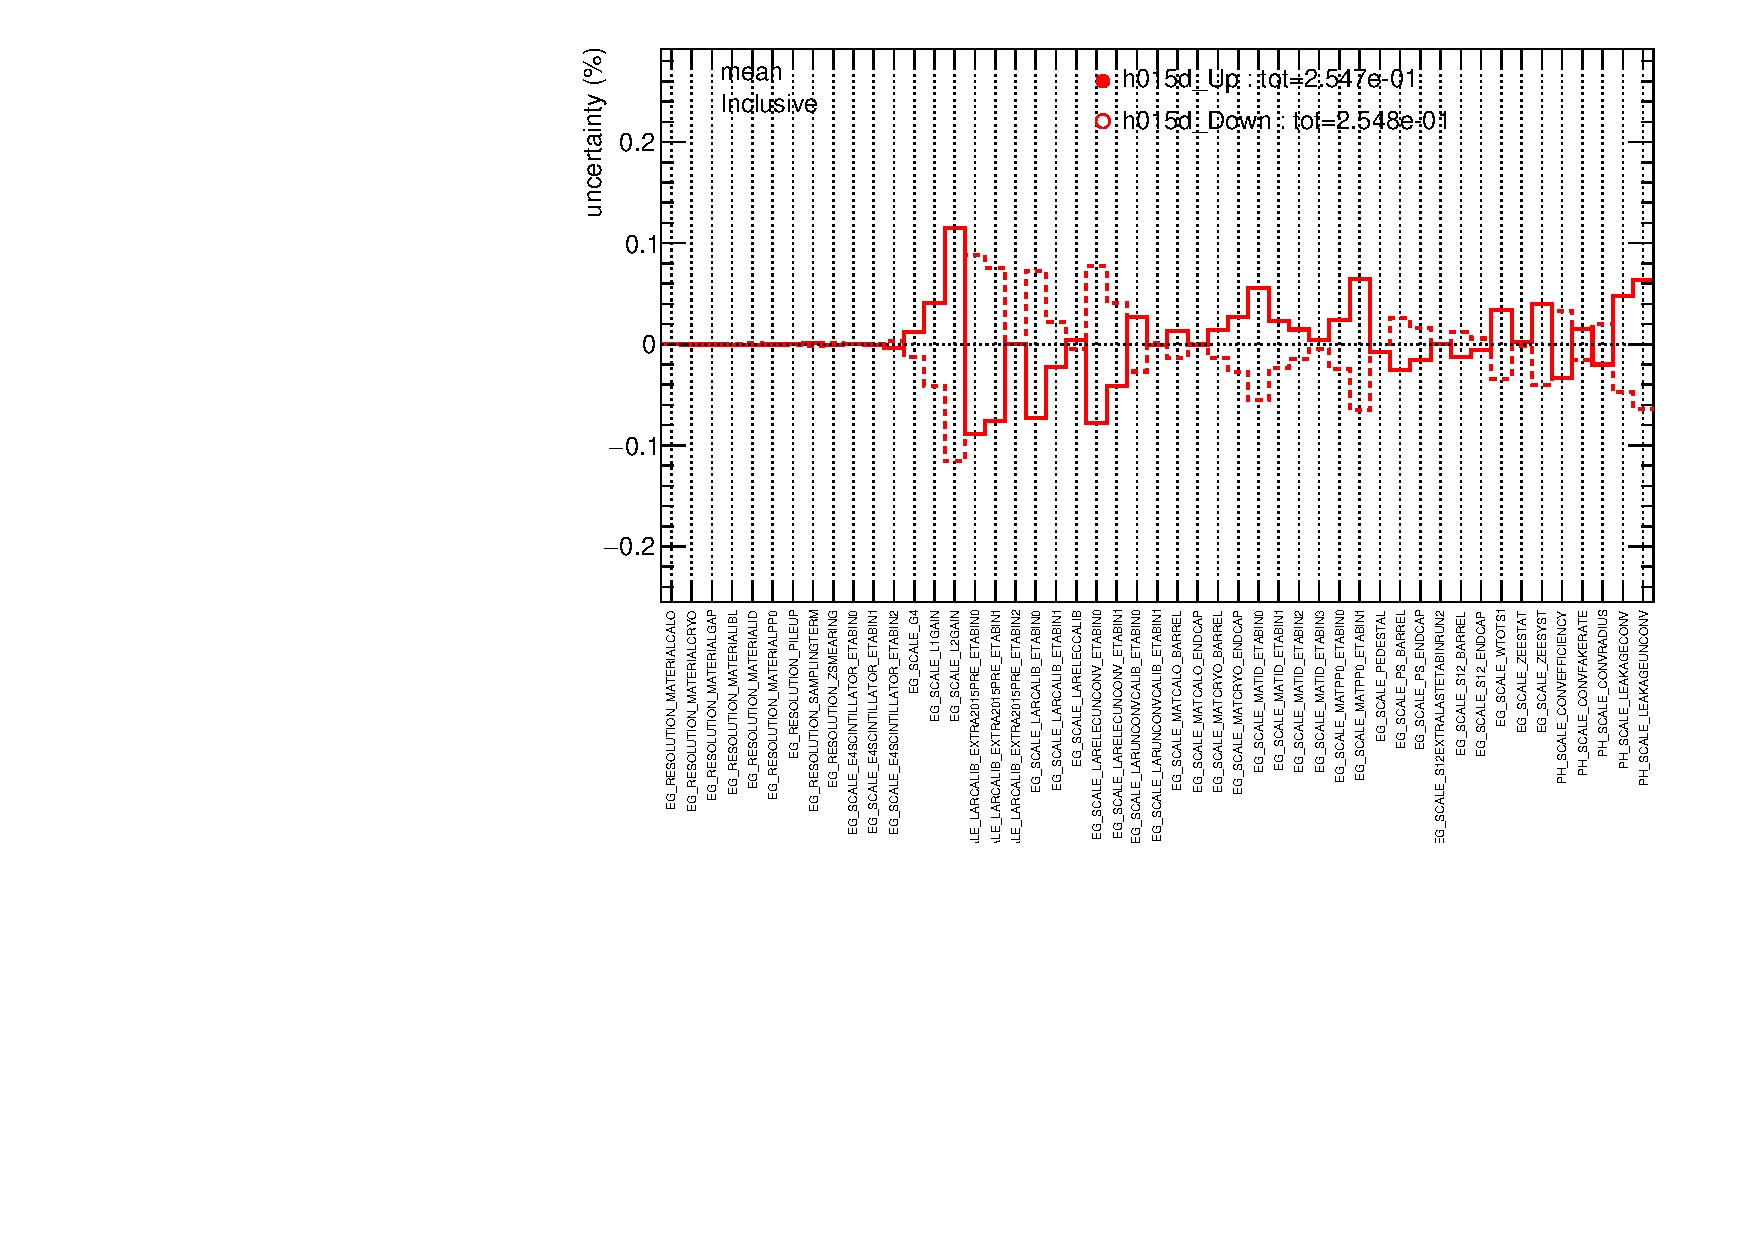
\includegraphics[width=\linewidth]{Figures/h015d_FULLMerge_catMerge_Systematics_Inclusive_mean_mean.pdf}
  \end{minipage}

  \begin{minipage}{0.49\linewidth}
    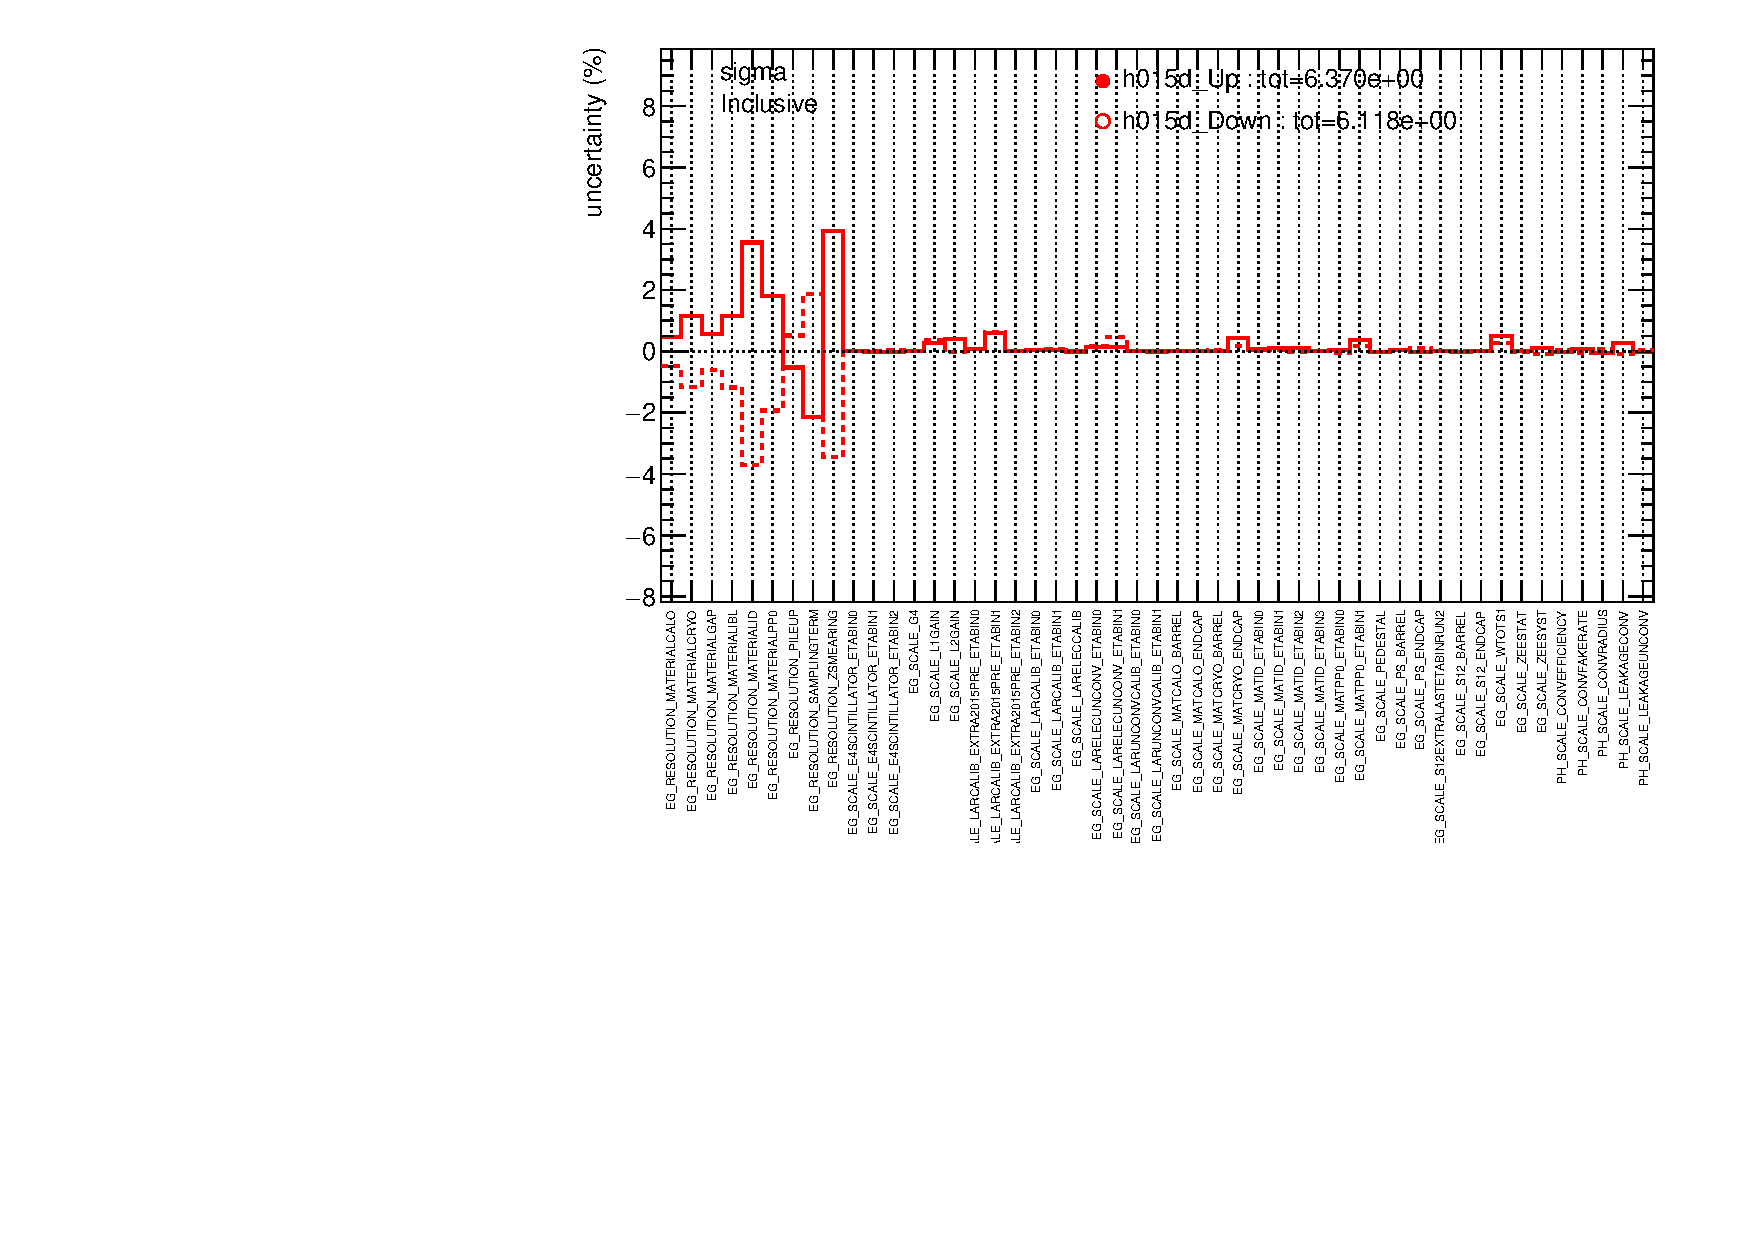
\includegraphics[width=\linewidth]{Figures/h015d_FULLMerge_catMerge_Systematics_Inclusive_sigma_sigma.pdf}
  \end{minipage}
  \hfill
  \begin{minipage}{0.49\linewidth}
    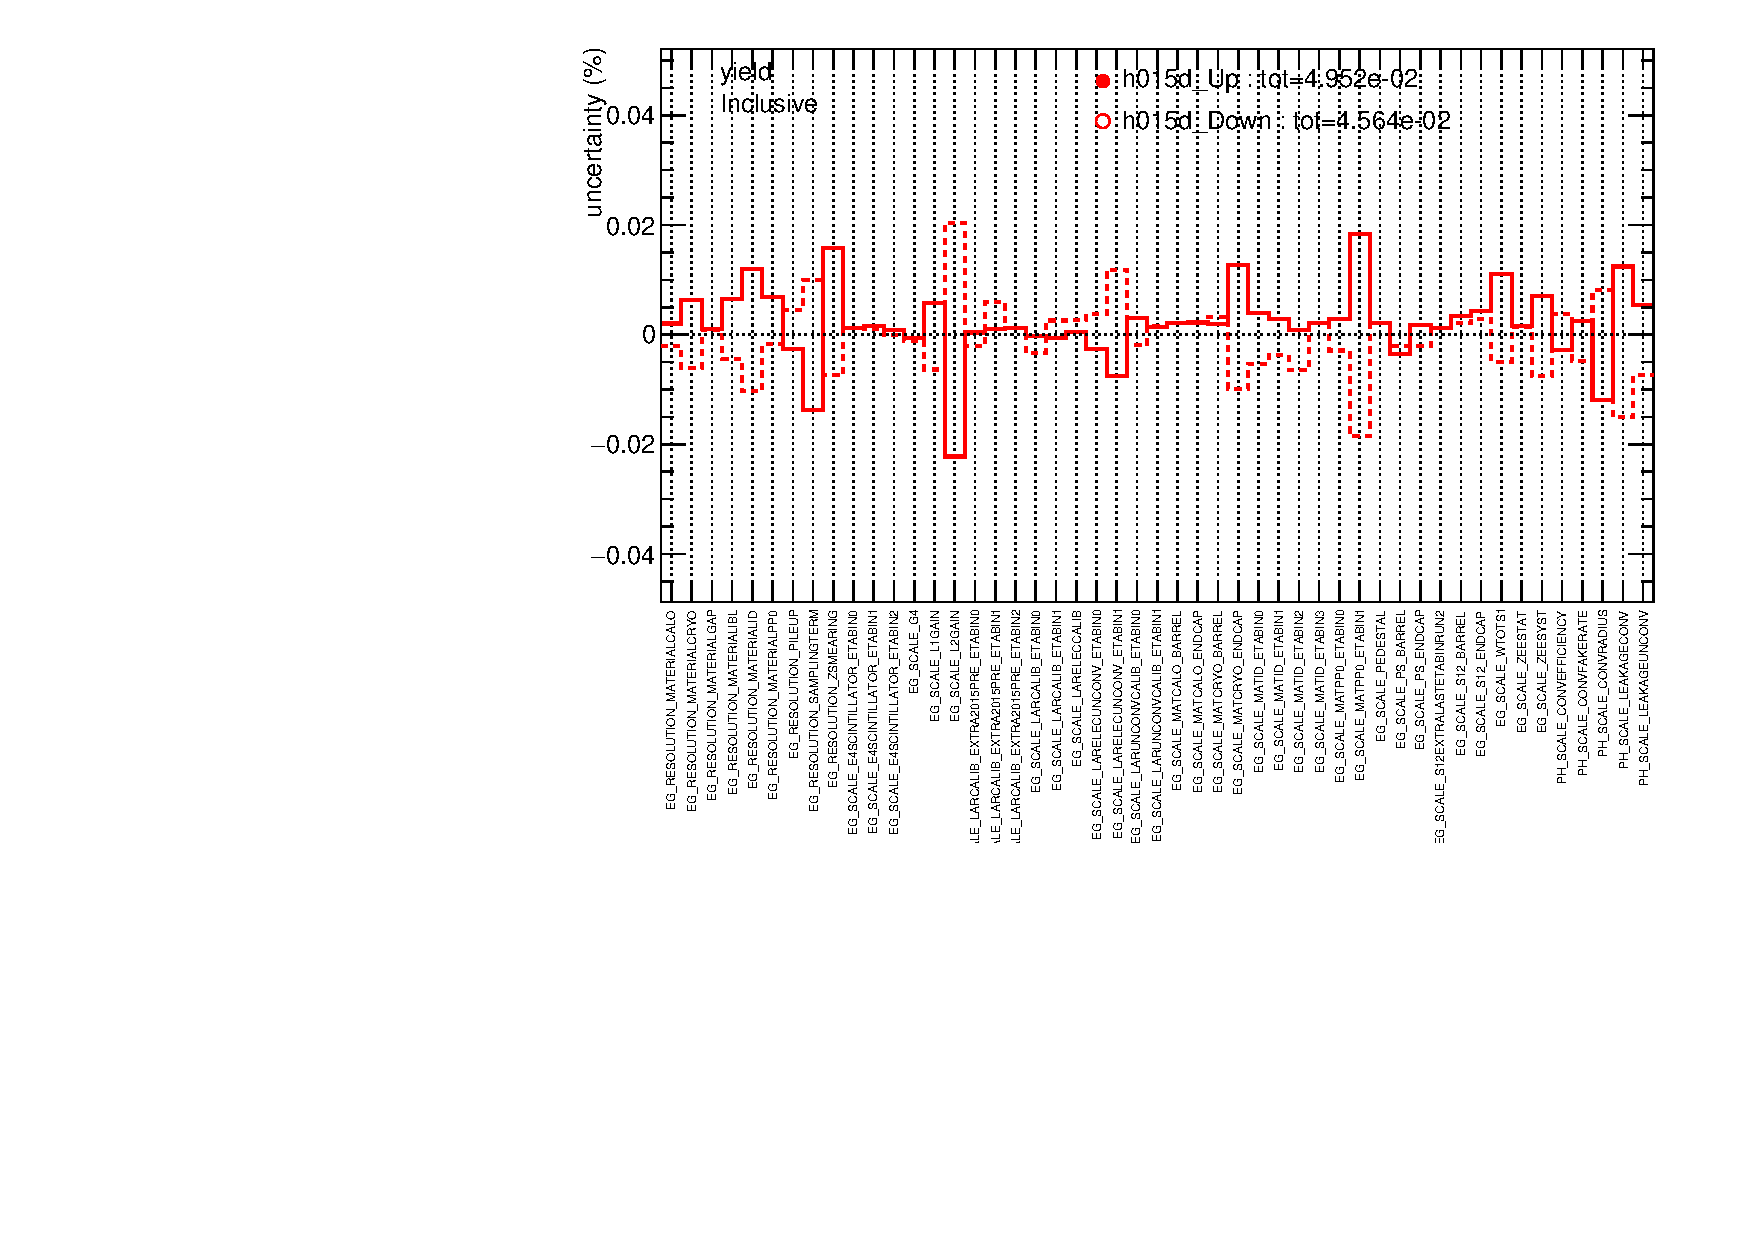
\includegraphics[width=\linewidth]{Figures/h015d_FULLMerge_catMerge_Systematics_Inclusive_yield_yield.pdf}
  \end{minipage}

\end{frame}
%%=================================================================================
\begin{frame}{Total uncertainty}
  \centering
  Total calibration uncertainty as a function of reconstructed category.\\
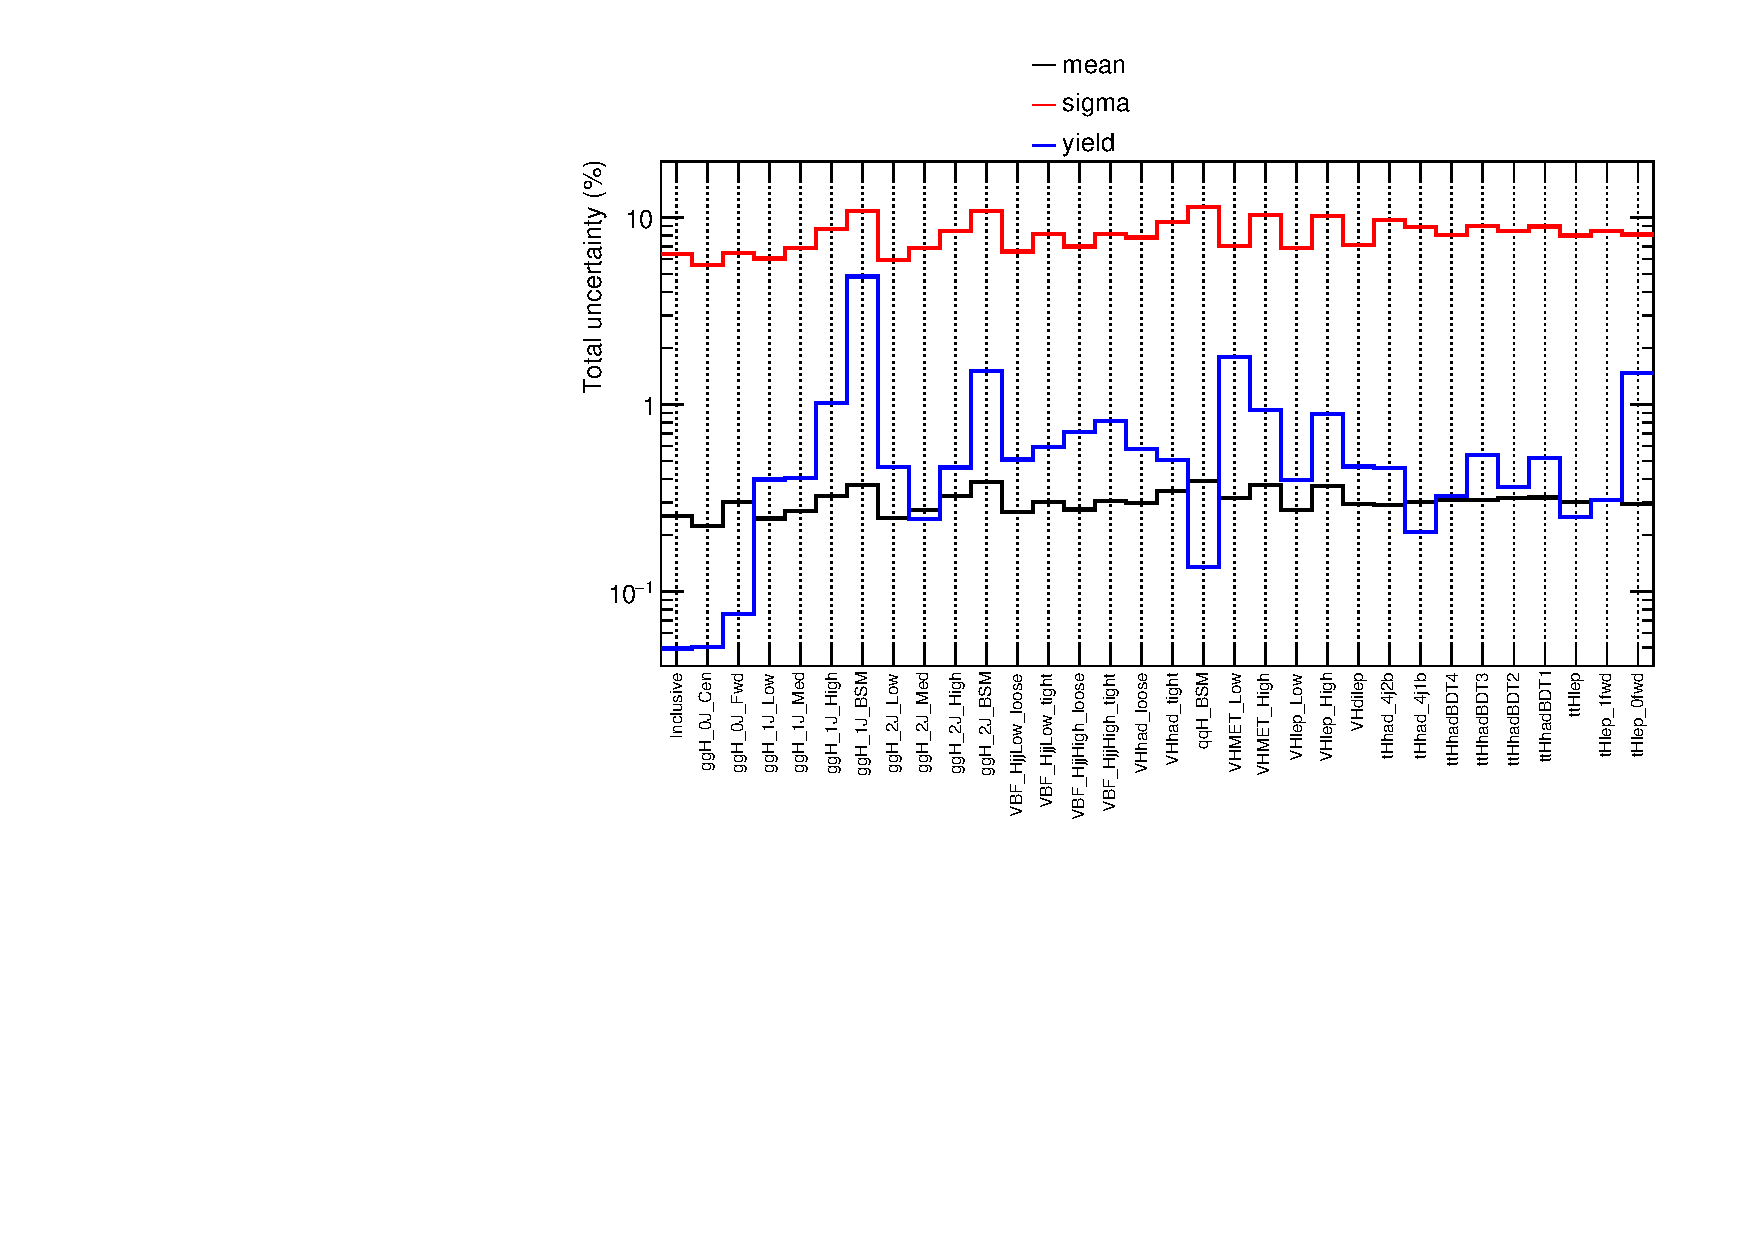
\includegraphics[width=0.9\linewidth]{Figures/h015d_FULLMerge_catMerge_Systematics_InclusiveUp.pdf}  
\end{frame}
%%=================================================================================
\begin{frame}{Likelihood Method}
A function ({\bf likelihood}) is built to {\bf evaluate the best set of parameters ($\vec{\mu}$,$\vec{\theta}$)} of a model to agree the best with a dataset in a category.

$$\mathcal{L}=\underbrace{\frac{(n_{s}(\vec{\mu},\vec{\theta})+b)^{n_{obs}}}{n_{obs}!} e^{-(n_{s}(\vec{\mu},\vec{\theta})+b)}}_{\textcolor{red}{\text{(1)}}}  \overbrace{\prod_j^{n_{obs}}\psi(\vec{x_j};\vec{\mu},\vec{\theta})}^{\textcolor{violet}{\text{(2)}}} \underbrace{e^{-\frac{\theta^2}{2}}}_{\textcolor{blue}{\text{(3)}}}$$
\vfill
\begin{minipage}{0.49\linewidth}
\textcolor{red}{(1) {\bf Poissonian law} to evaluate the probability to observe $n_{obs}$($\equiv$ signal $+$ background) events when $(n_s+b)$ are expected.}\newline
\textcolor{violet}{(2) {\bf Probability density function} of the observables $\vec{x}$ (diphoton invariant mass for example) for the $j^{th}$ event.}\newline
\textcolor{blue}{(3) Constraint on the nuisance parameter $\theta$. See next slide.}\newline
\end{minipage}
\begin{minipage}{0.49\linewidth}
\includegraphics[width=\linewidth]{Cgam_009.png}
\end{minipage}
\end{frame}
%%==========================================================

\begin{frame}{Nuisance parameters}
There are some {\bf external measurements}  that contribute to the likelihood and have some {\bf uncertainties}. 
A {\bf free nuisance parameter} is added for each of these measurements.
In order  to take into account these external measurements, a {\bf constraint is put on these nuisance parameters}. 
\vfill
For example, the luminosity is re-defined as  $L(1+\delta_L \theta_L)$, with $\theta_L$ the nuisance parameter and $\delta_L$ the uncertainty on the luminosity (assumed to be Gaussian).
In this case, a Gaussian constraint is chosen.

The contribution from luminosity will hence be :
$$L(1+\delta_L \theta_L)e^{-\theta_L^2/2}$$
\vfill
\textcolor{blue}{\bf Error Estimation}\newline
A test statistic is defined as : $t_\mu=-2ln\frac{\mathcal{L}(\mu,\hat{\hat{\theta}})}{\mathcal{L}(\hat{\mu},\hat{\theta})}$, with $\hat{\theta}$ and $\hat{\mu}$ the best (fitted) parameters, and $\hat{\hat{\theta}}$ the fitted nuisance parameters for a fixed $\mu$.\newline
Uncertainty are given by : \textcolor{red}{$\mathbf{t_{\hat{\mu}\pm 1\sigma}=1}$} and \textcolor{red}{$\mathbf{t_{\hat{\mu}\pm 2\sigma}=4}$} in 1D Gaussian limit.
\end{frame}
%%====================================================================

\begin{frame}{Run 2 couplings results}
  \centering
  Due to lack of statistics, some truth bins have been merged.
  \tiny 
  \begin{align*}
    \sigma (ggH, \mathrm{0~jet}) \tbfhyy &= 63\ ^{+17}_{-16}\ \fb  &= 63\ ^{+15}_{-15}\,\mathrm{(stat.)}\ ^{+8}_{-6}\,\mathrm{(syst.)}\ \fb \\
    \sigma (ggH, \mathrm{1~jet}, p_T^{H} < 60\ \text{GeV}) \tbfhyy &= 15\ ^{+13}_{-12}\ \fb  &= 15\ ^{+12}_{-12}\,\mathrm{(stat.)}\ ^{+6}_{-4}\,\mathrm{(syst.)}\ \fb \\
    \sigma (ggH, \mathrm{1~jet}, 60 \leq p_T^{H} < 120\ \text{GeV}) \tbfhyy &= 10\ ^{+7}_{-6}\ \fb  &= 10\ ^{+6}_{-6}\,\mathrm{(stat.)}\ ^{+2}_{-1}\,\mathrm{(syst.)}\ \fb \\
    \sigma (ggH, \mathrm{1~jet}, 120 \leq p_T^{H} < 200\ \text{GeV}) \tbfhyy &= 1.7\ ^{+1.7}_{-1.6}\ \fb  & = 1.7\ ^{+1.6}_{-1.6}\,\mathrm{(stat.)}\ ^{+0.6}_{-0.4}\,\mathrm{(syst.)}\ \fb \\
    \sigma (ggH, \geq 2~\mathrm{jet}) \tbfhyy &= 11\ ^{+8}_{-8}\ \fb  &= 11\ ^{+8}_{-8}\,\mathrm{(stat.)}\ ^{+3}_{-2}\,\mathrm{(syst.)}\ \fb \\
    \sigma (qq \rightarrow Hqq, p_T^{j} < 200~\text{GeV}) \tbfhyy &= 10\ ^{+6}_{-5}\ \fb  &= 10\ ^{+5}_{-5}\,\mathrm{(stat.)}\ ^{+2}_{-1}\,\mathrm{(syst.)}\ \fb \\
    \sigma (ggH + qq \rightarrow Hqq, \mathrm{BSM-like}) \tbfhyy &= 1.8\ ^{+1.4}_{-1.4}\ \fb  &= 1.8\ ^{+1.3}_{-1.3}\,\mathrm{(stat.)}\ ^{+0.5}_{-0.5}\,\mathrm{(syst.)}\ \fb \\
    \sigma (\mathrm{VH, leptonic}) \tbfhyy &= 1.4\ ^{+1.4}_{-1.2}\ \fb  &= 1.4\ ^{+1.3}_{-1.2}\,\mathrm{(stat.)}\ ^{+0.3}_{-0.3}\,\mathrm{(syst.)}\ \fb \\
    \sigma (\mathrm{top}) \tbfhyy &= 1.3\ ^{+0.9}_{-0.8}\ \fb  &= 1.3\ ^{+0.9}_{-0.8}\,\mathrm{(stat.)}\ ^{+0.3}_{-0.1}\,\mathrm{(syst.)}\ \fb \\
\end{align*}

\end{frame}
%%====================================================================
\begin{frame}{Run 2 signal strength results}
  STXS difficult to interpret directly.\\
  Measurement of signal strengths $\mu_i = \frac{\sigma_i^{exp}}{\sigma_i^{SM}}$ performed.\\

  \begin{minipage}{0.49\linewidth}
    \includegraphics[width=\linewidth]{ATLAS-CONF-2017-045_11f.pdf}
  \end{minipage}
  \hfill
  \begin{minipage}{0.49\linewidth}
    \centering
    \includegraphics[width=0.7\linewidth]{ATLAS-CONF-2017-045_6t.pdf}
  \end{minipage}

  \begin{center}
  \begin{minipage}{0.49\linewidth}
    \begin{itemize}
    \item Major theory improvement
    \item Major resolution improvement
    \item Increase of mass scale impact
    \item   \textcolor{red}{\bf No deviation from SM}
      \end{itemize}
  \end{minipage}

  \end{center}
\end{frame}
